\chapter{Longitudinal stability of an aircraft}
% introduzione... stabilità, grafici e quali sono tutti i dati che servono

\section{Aerodynamic Lift}
% intro
\subsection{Wing}
\subsection{Fuselage}
\subsection{Horizontal Tail}
\subsubsection{Elevator index of effectiveness}
 In order to evaluate the contribution to the longitudinal stability of horizontal tail it's necessary to consider the deflection of the elevator. 
		
		 %disegno elevatore --> p 95 pgv
		
The variation of zero lift angle is not constant with the angle of deflection. So it's necessary to evaluate the tau factor which is defined as follows:

\begin{equation}		 
\tau_e = \frac{d \alpha_{0l}}{d \delta_e}
\end{equation}

		
Introducing this parameter the lift coefficient of the horizontal tail can be rated as follows:

\begin{equation}
C_{L_H}= C_{L_0} + C_{L_{{\alpha}_H}} \alpha_H + 	C_{L_{{\alpha}_H}} \tau_e \delta_e
\end{equation}

  
Considering a symmetrical horizontal tail, the term $C_{L_0}$ is zero, so it's possible to express the lift coefficient in the following form:


\begin{equation}
C_{L_H}= C_{L_{{\alpha}_H}} \left ( \alpha_H + \tau_e \delta_e \right)
\end{equation}
  		
 In general the value of $\tau$ is constant until about 15 deg; after this value, due to the flow separation, the effectiveness of elevator decrease and consequently the product $ \tau_e \delta_e$ that appears in the equation of lift coefficient.
		
%grafici di progetto.
		
The evaluation of tau is made by reading of external database, considering the following graphs.
	
\begin{equation}
\tau = \alpha_{\delta} \eta_{\delta} = \frac{\alpha_{{\delta}_{c_L}}}{\alpha_{{\delta}_{c_l}}}\alpha_{{\delta}_{c_l}} \eta_{\delta}
\end{equation}



\begin{figure}[H]
\centering
{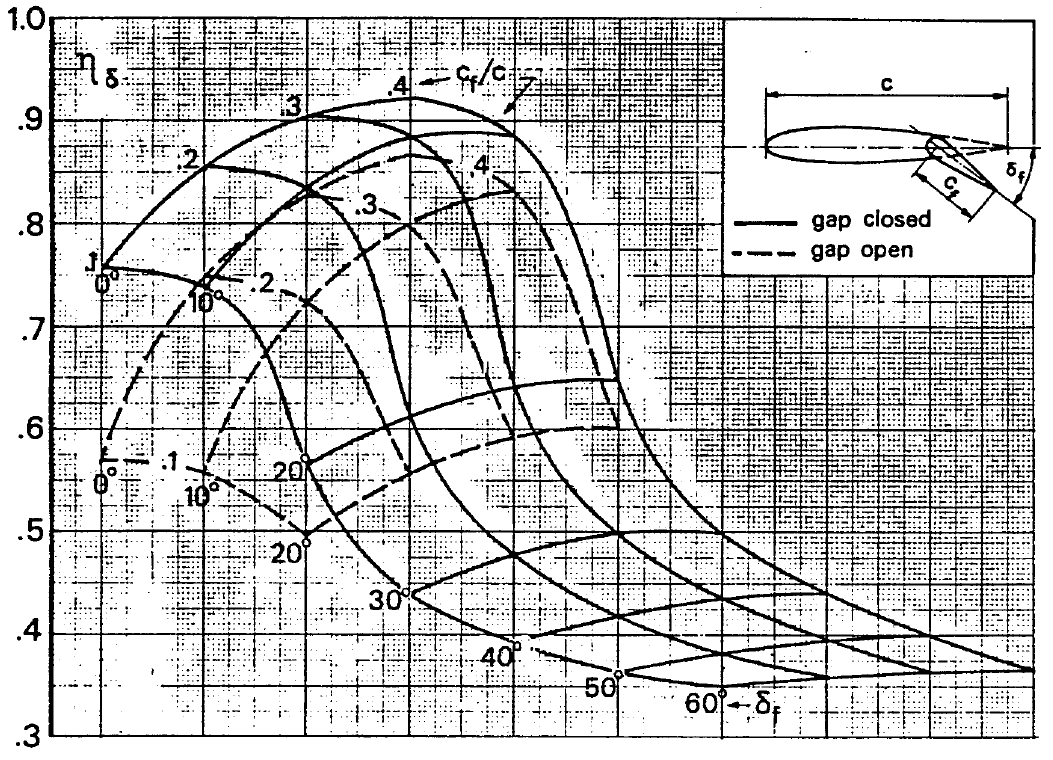
\includegraphics[height=6cm]{Immagini/Eta_Delta_Plain.png}} 
\caption{2D efficiency correction for elevator.}
\label{efficiency}
\end{figure} 		


\begin{figure}[H]
\centering
{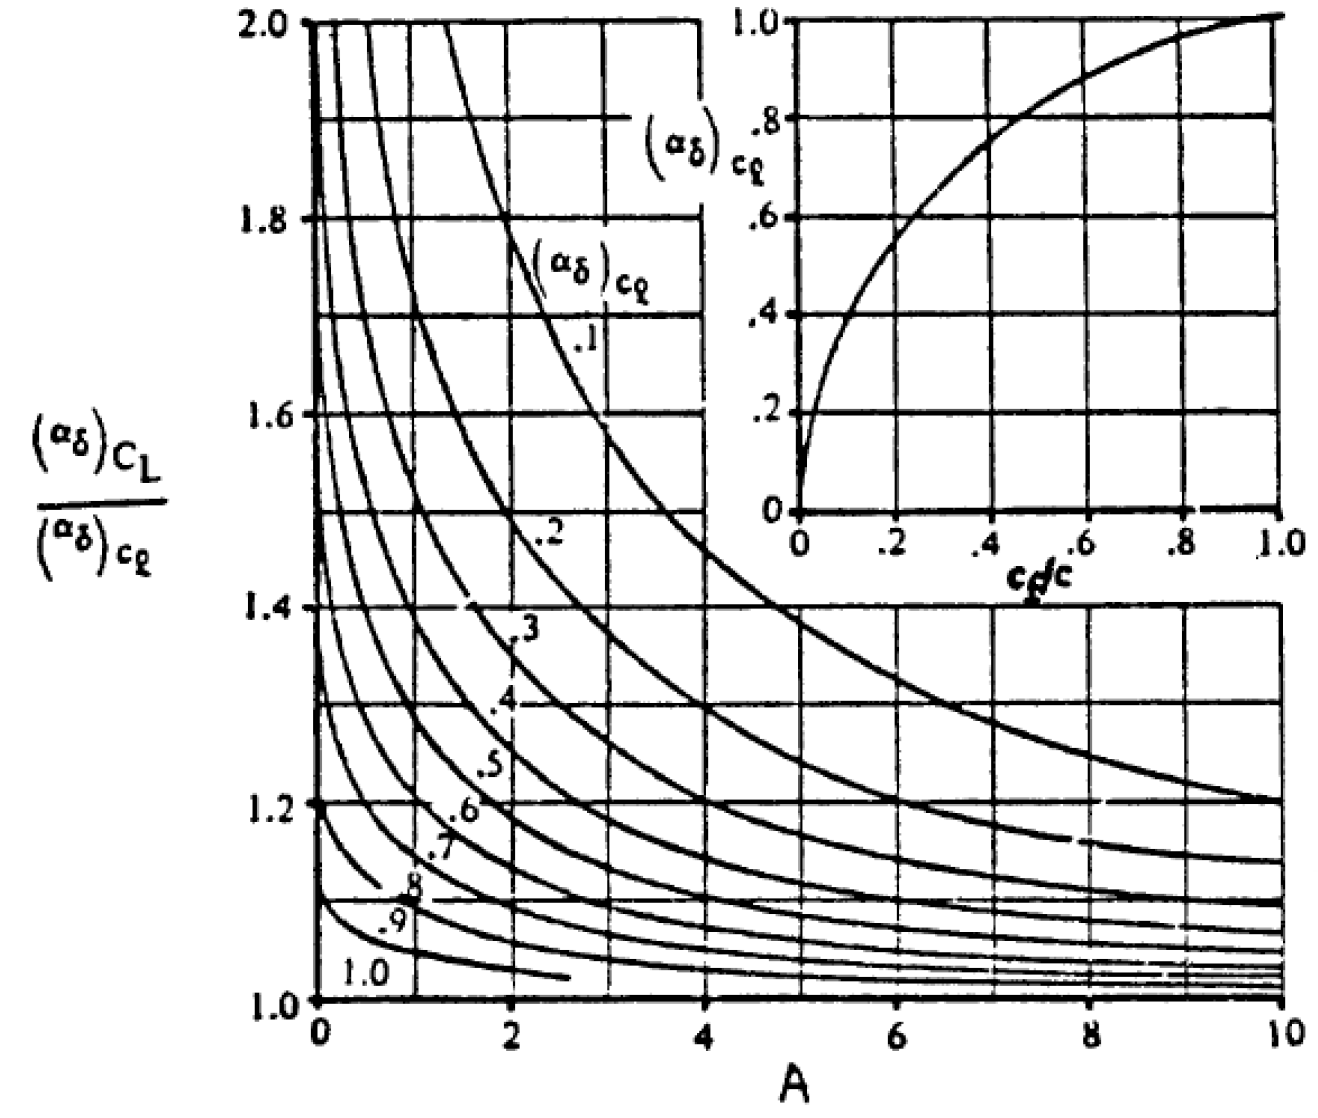
\includegraphics[height=6cm]{Immagini/alfadelta.png}} 
\caption{$\frac{d \alpha_{0l}}{d \delta_e}$ 2D and 3D correction.}
\label{efficiency}
\end{figure} 		
		
\subsubsection{Developer's Guide} % java class archiecture(?)
%tabella elenco metodi con classe e che fanno

% descrizione

% spiegazione  (da fare) del calcolo del cl at alfa simile a quello dell ala
% spiegazione (da fare )  metodo calcolo tau in stability calculator
% spiegazione (gia fatta) del metodo calculateclwithdeflection in ls aerodynamic

% grafici con risultati

\subsection{Complete Aircraft}

\section{Aerodynamic Drag}

\section{Pitching Moments}
\subsection{Wing}
\subsection{Fuselage}
\subsection{Horizontal Tail}
\subsection{Propulsors}

\subsection{Stability Calculation}
% calcolo delle forze normali e tangenziali, calcolo momenti, risultati